\documentclass[11pt]{report}
\usepackage{textcomp}

\usepackage{titlesec}
\titlespacing*{\section}
{0pt}{\baselineskip}{0em}
\titlespacing*{\subsection}
{0pt}{\baselineskip}{0em}

\usepackage{geometry}
\geometry{left=1in, right=1in, top=1in, textheight=9in}

\usepackage{enumitem}
\newlist{steps}{enumerate}{1}
\setlist[steps, 1]{wide=0pt, leftmargin=\parindent, label=Step \arabic*:}

\usepackage{fancyhdr}
\fancypagestyle{plain}{%
    \fancyhf{} % clear all header and footer fields
    \fancyfoot[C]{\sffamily\fontsize{.75em}{.75em}\selectfont\thepage} % except the center
    \renewcommand{\headrulewidth}{0pt}
    \renewcommand{\footrulewidth}{0pt}
}
\pagestyle{plain}

\usepackage{graphicx}
\graphicspath{ {./media/} }

\usepackage{setspace}
\doublespacing

\usepackage{minted}
\usepackage{xcolor}
\definecolor{LightGray}{gray}{0.9}
% \newmintinline[vhdl]{vhdl}{fontsize=\small, bgcolor=LightGray}

% make fancy title page
\makeatletter
\newcommand{\@labsection}{000}
\newcommand{\labsection}[1]{
    \renewcommand{\@labsection}{#1}
}

\newcommand{\@labnumber}{0}
\newcommand{\labnumber}[1]{
    \renewcommand{\@labnumber}{#1}
}

\newcommand{\@shortsubmitted}{1/1/70}
\newcommand{\shortsubmitted}[1]{
    \renewcommand{\@shortsubmitted}{#1}
}

\lfoot{\footnotesize \textit{University of Arkansas \\ EECS Department}}
\rfoot{\footnotesize \textsl{\@shortsubmitted}}

\renewcommand{\maketitle}{
    \newgeometry{left=1in, right=1in, top=1.75in, textheight=8.25in}
    \singlespacing
    \begin{center}
        {\huge \bf CSCE 22104} \\
        \vspace{2.5em}
        {\Large \bf Lab Report} \\
        \vspace{2em}
        \noindent\rule{20em}{0.4pt} \\
        \vspace{1em}
        {\Large \@author} \\
        \vspace{.75em}
        {\normalsize ID: 011019116} \\
        \vspace{.75em}
        {\normalsize Lab Section \@labsection} \\
        \vspace{.75em}
        {\normalsize Lab \@labnumber} \\
    \end{center}
    \newpage
    \restoregeometry
}

\makeatother


% TEXTWIDTH = 100
\begin{document}
\title{Lab Report 6}
\author{Brent Marcus Orlina}

\labsection{001}
\labnumber{6}

\shortsubmitted{3/19/25}

\maketitle

\section*{Introduction}
This lab's goal was to create a 1-bit ALU component and create a 16-bit ALU component, using 1-bit
components. The ALU components should support four operations: addition, subtraction, logical-and,
and logical-or, using the opcodes \verb|00|, \verb|01|, \verb|10|, and \verb|11|, respectively. The
components should also be asynchronous, i.e. the component does not depend on a clock.

\section*{Approach}
\begin{listing}[h!]
    \inputminted[
        frame=lines,
        breaklines,
        linenos,
        tabsize=4,
        fontsize=\footnotesize,
        bgcolor=LightGray
    ]{vhdl}{./media/ALU1Bit-port.vhd}
    \caption{The 1-bit ALU component's ports.}
    \label{listing:ALU1Bit-port}
\end{listing}

The 1-bit ALU component was first implemented. Listing \ref{listing:ALU1Bit-port} shows the ports
that the ALU takes in. The input port \verb|s| represents the opcode, determining wether the ALU
should execute an addition, subtraction, logical-and, or logical-or operation. The input ports
\verb|a| and \verb|b| are the operands. The input port \verb|cin| is the carry-in from a previous
ALU component, used for the addition and subtraction operations. It is unused when performing a
logical-and or a logical-or operation.

The output port \verb|sout| is the result of the operation that was executed. Output port
\verb|cout| is used for addition and subtraction operations, connected to the next ALU component so
that it can correctly calculate the result. Although \verb|cin|s and \verb|cout|s are not used for
the logical-and and logical-or operations, it will still be calculated regardless. It will not
affect the result since the two logical operations do not use the \verb|cin| input port.

\newpage

\begin{listing}[h!]
    \inputminted[
        frame=lines,
        breaklines,
        linenos,
        tabsize=4,
        fontsize=\footnotesize,
        bgcolor=LightGray
    ]{vhdl}{./media/ALU1Bit-datapath.vhd}
    \caption{The 1-bit ALU component's datapath implementation.}
    \label{listing:ALU1Bit-datapath}
\end{listing}

Listing \ref{listing:ALU1Bit-datapath} shows the implementation for each of the operations that the
ALU supports. Firstly, the signals \verb|sout_adder|, \verb|sout_and|, and \verb|sout_or|,
correspond to the results of each operations that the ALU supports, with \verb|sout_adder|
corresponding to both the addition and subtraction operations. The signal \verb|inverse_b| is used
to support subtraction. The results of all of the operations are calculated with the input port
\verb|s| deciding which result to connect to the output port \verb|sout| by using the operations'
respective opcodes.

Notice that since the result of addition and subtraction operations both correspond to only one
signal. This allows it so that only the $1^{st}$ bit is checked to be a $0$ since both operations'
opcodes have their $1^{st}$ as a $0$. The motivation behind merging both operations into one signal
is that binary subtraction in twos complement is equivalent to
\begin{equation} \label{eq:binary_subtraction}
    A - B = A + (\widetilde{B} + 1)
\end{equation}
therefore, the input port \verb|b| must simply be inverted to support the subtraction operation.
Since the addition and subtraction's opcodes are different in the $0^{th}$ bit where subtraction has
a $1$, \verb|b| can simply be \verb|XOR|ed by the $0^{th}$ bit of the opcode, which inverses
\verb|b| when the opcode signals for a subtraction operation. This potential inverse of \verb|b| is
connected to the \verb|inverse_b| signal, used only by the addition and subtraction operations, so
that it does not affect the other operations in which the $0^{th}$ bit of the opcode is a $1$.

The addition of the extra $1$ to $\widetilde{B}$ in \ref{eq:binary_subtraction} is not implemented
in the 1-bit ALU since if the 16-bit ALU was implemented using sixteen 1-bit ALUs, it would add an
extra 1 in each bit of the 16-bit ALU, producing the wrong result. The extra $1$ will come from the
\verb|cin| of the first 1-bit ALU, again using the $0^{th}$ bit of the opcode, later shown in [REF
to later figure here]. 

The addition operation remains correct as the input port \verb|b| won't be inverted and there
won't be an extra addition of one since the $0^{th}$ bit of the opcode will be $0$. The other two
operations, logical-and and logical-or, are trivial by simply performing an \verb|AND| or an
\verb|OR| between input ports \verb|a| and \verb|b|. The \verb|cout| output port is also somewhat
trivial, implemented similarly to a normal Full Adder. However, it uses the signal \verb|inverse_b|
to support subtraction.

\begin{listing}[h!]
    \inputminted[
        frame=lines,
        breaklines,
        linenos,
        tabsize=4,
        fontsize=\footnotesize,
        bgcolor=LightGray
    ]{vhdl}{./media/ALU16Bit-port.vhd}
    \caption{The 16-bit ALU component's ports.}
    \label{listing:ALU16Bit-port}
\end{listing}

Now that the 1-bit ALU has been implemented, the 16-bit ALU can now be constructed using sixteen
1-bit ALU components. Listing \ref{listing:ALU16Bit-port} shows the 16-bit ALU component's ports.
Notice that the input ports \verb|a| and \verb|b| and the output port \verb|sout| are now
\verb|std_logic_vector|s with 16 bits each, since the data will be 16 bits long. The input port
\verb|s| is unchanged as it still corresponds to the opcode. The output port \verb|cout| also
reamins unchanged as it will be the \verb|cout| of the last 1-bit ALU component.

\newpage

\begin{listing}[h!]
    \inputminted[
        frame=lines,
        breaklines,
        linenos,
        tabsize=4,
        fontsize=\footnotesize,
        bgcolor=LightGray
    ]{vhdl}{./media/ALU16Bit-datapath.vhd}
    \caption{The 16-bit ALU component's datapath implementation.}
    \label{listing:ALU16Bit-datapath}
\end{listing}

Listing \ref{listing:ALU16Bit-datapath} shows the implementation of the 16-bit ALU component, using
a sixteen 1-bit ALU components. The opcode, in the input port \verb|s|, is connected to all of the
1-bit ALU components since each 1-bit ALU component needs to know the operation to execute. Each bit
of the input ports \verb|a| and \verb|b| as well as the output port \verb|sout| are connected to the
corresponding 1-bit ALU component.

To make the addition and subtraction operations work correctly, a 1-bit ALU component's \verb|cout|
output port must be connected to the next 1-bit ALU component's \verb|cin| input port, acting as the
carry. The last 1-bit ALU component's \verb|cout| output port is connected to the 16-bit ALU
component's \verb|cout|. The first 1-bit ALU component's \verb|cin| is connected to the $0^{th}$ bit
of the opcode. This is because if the operation to be executed is subtraction, which has the opcode
of \verb|01|, must have an extra $1$ added as shown in equation \ref{eq:binary_subtraction}. If the
operation is addition, the opcode would be \verb|00|, thus not adding an extra $1$, correctly
calculating the result. The other two operations do not use the \verb|cin| and \verb|cout| ports,
correctly calculating the results bit by bit.


\section*{Experimentation}
Both components were individually tested using a testbench. The 1-bit ALU component was tested by
going through all of the operations, each with all possible combinations of the input ports
\verb|a|, \verb|b| and \verb|cin|. The 16-bit ALU component was tested with a given list of inputs
and manually verifying that the outputs are correct.

\section*{Results \& Discussion}
\begin{figure}[h!]
    \centering
    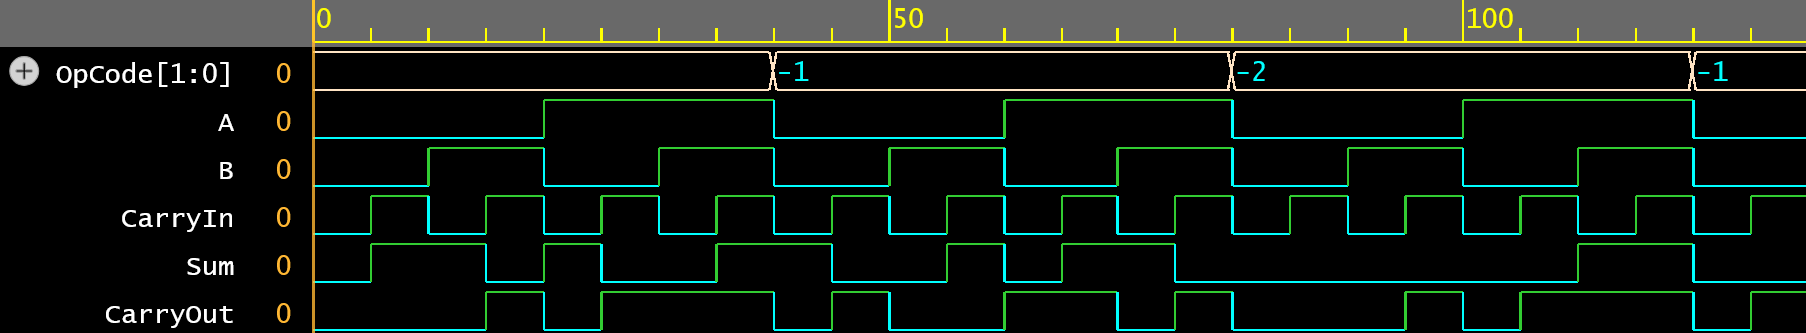
\includegraphics[width=0.95\textwidth]{ALU1Bit-waveform}
    \caption{The waveform for the 1-bit ALU component.}
    \label{fig:ALU1Bit-waveform}
\end{figure}

The 1-bit ALU component works as expected. Figure \ref{fig:ALU1Bit-waveform} shows the waveform of
the 1-bit ALU component, correctly outputting the results of each operation. For the subtraction
operation, it is noteworthy that the output is unintuitive, especially shown when the signals
\verb|A|, \verb|B|, and \verb|CarryIn| are all zeroes while the output shows the signal \verb|Sum|
to be active. This is because \verb|B| is being inverted and then being "added" to zeroes, resulting
in \verb|Sum| to be active. Though the implementation results in this peculiarity, it is required
for the 16-bit ALU to work.

\begin{figure}[h!]
    \centering
    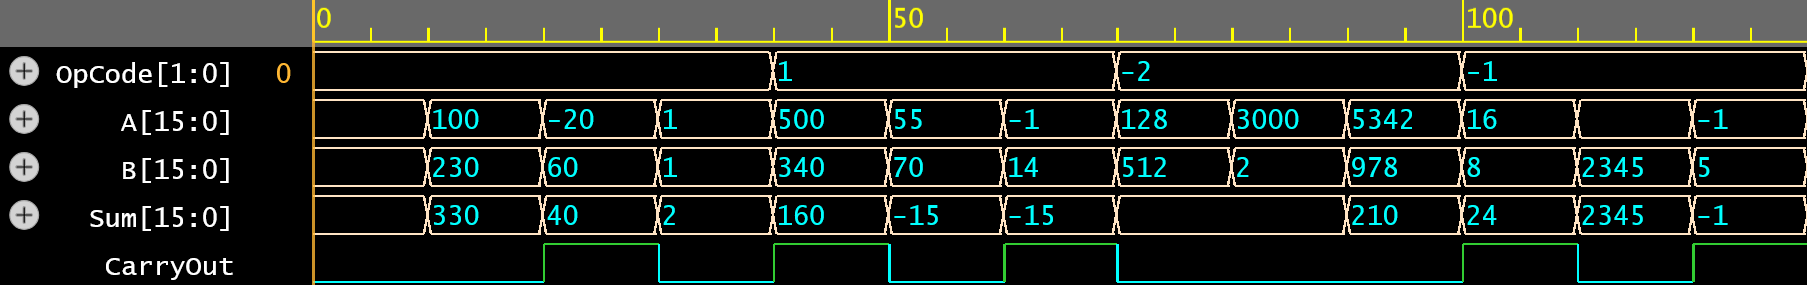
\includegraphics[width=0.95\textwidth]{ALU16Bit-waveform}
    \caption{The waveform for the 16-bit ALU component. Signals that display a blank are zeroes.}
    \label{fig:ALU16Bit-waveform}
\end{figure}

\begin{table}[ht!]
    \centering
    \begin{tabular}{|cc||cc|c|c|} 
     \hline
     S1 & S0 & A & B & Sout & Cout \\
     \hline
     0 & 0 & 100 & 230 & 330 & 0 \\ 
     \hline
     0 & 0 & -20 &  60 &  40 & 1 \\
     \hline
     0 & 0 &   1 &   1 &   2 & 0 \\
     \hline
     %             
     0 & 1 & 500 & 340 & 160 & 1 \\ 
     \hline
     0 & 1 &  55 &  70 & -15 & 0 \\
     \hline
     0 & 1 &  -1 &  14 & -15 & 1 \\
     \hline
     %             
     1 & 0 &  128 & 512 &   0 & 0 \\ 
     \hline
     1 & 0 & 3000 &   2 &   0 & 0 \\
     \hline
     1 & 0 & 5342 & 978 & 210 & 0 \\
     \hline
     %             
     1 & 1 & 16 &    8 &   24 & 1 \\ 
     \hline
     1 & 1 &  0 & 2345 & 2345 & 0 \\
     \hline
     1 & 1 & -1 &    5 &   -1 & 1 \\
     \hline
    \end{tabular}
    \caption{Results of the 16-bit ALU component testbench in table form.}
    \label{table:ALU16Bit-waveform_table}
\end{table}

The 16-bit ALU component works as expected. Figure \ref{fig:ALU16Bit-waveform} shows the waveform of
the 16-bit ALU component, correctly outputting the results of each operation. The waveform also
displays the signal \verb|OpCode| in signed decimal, with the signals \verb|-2| and \verb|-1|
corresponding to the opcodes \verb|10| and \verb|11| respectively. Table
\ref{table:ALU16Bit-waveform_table} shows the waveform results in table form.


\section*{Conclusions}
Both the 1-bit ALU and 16-bit ALU components worked correctly and displayed the expected behavior
during testing. The knowledge learned from this lab was learning how to construct 1-bit ALU
component that handled multiple operations determined by an opcode. Learning how subtraction works
in binary was also a part of the lab, as well as learning how to construct a 16-bit ALU component
using out of 1-bit ALU components.
% \newpage
% 
% \section*{References}
% \noindent
% [1]    Computer Organization 22104, EECS, University of Arkansas, “Lab 1,”  Sep. 17, 2024.
% 
% \noindent
% [2]    Computer Organization 22104, EECS, University of Arkansas, “Lab 2,”  Sep. 24, 2024.
% 
% \newpage
% 
% \section*{Appendix}
% \begin{figure}[h!]
%     \centering
%     \includegraphics[width=0.9\textwidth]{foo}
%     \caption{
%         Lorem ipsum dolor sit amet, qui minim labore adipisicing minim sint cillum sint consectetur
%         cupidatat.
%     }
%     \label{fig:foo}
% \end{figure}
% 
% \newpage
% 
% \begin{figure}[h!]
%     \centering
%     \includegraphics[height=0.4\textheight]{bar}
%     \caption{Lorem ipsum something something shorter sentence}
%     \label{fig:bar}
% \end{figure}
\end{document}
